\newgeometry{margin=5mm}
\thispagestyle{empty}
\noindent
\begin{minipage}{30mm}
	\raisebox{-.5\totalheight}{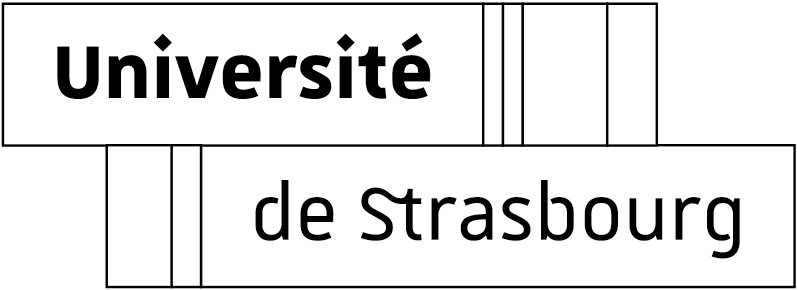
\includegraphics[width=\linewidth]{Logo/logo_unistra}}  
\end{minipage}
\begin{minipage}{.67\linewidth}\centering
	\vspace{1cm}
	{\large \textbf Farid \textsc{OUHMICH}}\\\vspace{.5cm}
	{ \textbf \textsc{}}

\end{minipage}
\begin{minipage}{30mm}
	\raisebox{-.5\totalheight}{
\includegraphics[width=0.5\linewidth]{Logo/ihu}}  
\end{minipage}
\vspace{0.2cm}

\noindent
\fbox{
	\renewcommand{\baselinestretch}{0.5}
	
	\begin{minipage}{0.97\linewidth}
		{\large  \textbf {Abstract}}
		
	\medskip
		{\small To evaluate the status of a liver tumor, we usually perform a biopsy followed by an anatomo-pathological evaluation of the extracted sample. However, the biopsy, due to the small sampling size, does not testify the intra and inter-tumor heterogeneity, thus struggling in assessing precisely the phenotypical characteristics of the patients.
		Recent progress in medical imaging and data science fields enabled the emergence of a new technique called radiomics, that is partially answering these challenges.
		In this thesis, we have been focusing on hepatocellular carcinoma, and we built new imaging methods to characterize this widespread pathology.
		By incorporating temporal information through multiphase images, specialized UNet-like networks have been stacked in a cascaded architecture to provide a semantic segmentation of both the liver and its internal tissue (parenchyma, active \& necrotic part of the tumor).
		To characterize the strong heterogeneity that resides in the tumor, we predict the histological grade on a fine scale (slice-wise), by re-using the features learned from the semantic segmentation network. Our preliminary results enable the production of a fine-detailed map of the tumor that separates well differentiated areas from poorly ones. 
		Even though these results need to be confirmed with a larger cohort, we believe that medical images combined with deep modeling techniques may soon be introduced in a clinical workflow to help diagnose and evaluate the phenotypical characteristics of pathologies such as liver cancer.
		}
		
	\medskip
		
	\textbf{Keywords}:  Liver cancer, Hepatocellular Carcinoma, Histological grade, Contrast Enhanced CT, Deep Learning, Semantic Segmentation,  Radiomics
	\end{minipage}
}

\vspace{0.5cm}

\noindent
\fbox{
	\renewcommand{\baselinestretch}{0.5}
	\begin{minipage}{.97\linewidth}
			{\large  \textbf {R\'{e}sum\'{e}}}
		%		\end{center}
		
		\medskip
		
		{\small Afin de caractériser une tumeur hépatique, une biopsie est le plus souvent réalisée, suivie d'une analyse anatomo-pathologique des tissus prélevés. Cependant, en raison de la faible taille des tissus prélevés, la biopsie ne permet pas de rendre compte de l'hétérogénéité intra et inter-patient, d'où sa difficulté à estimer précisément les caractéristiques phénotypiques des patients. Les progrès récents en imagerie médicale et en science des données ont permis l'émergence d'une nouvelle technique nommée radiomique, qui répond en partie à ces problématiques. Dans cette thèse, nous nous sommes intéressés aux hépatocarcinomes cellulaires, et nous avons implémentés de nouvelles méthodes d'imagerie pour caractériser cette pathologie. En incorporant l'information multiphase, des réseaux de neurones spécialisés de type U-Net ont été empilés en cascade pour effectuer une segmentation sémantique du foie et de ses différentes structures (parenchyme, parties active \& nécrotique de la tumeur). Pour caractériser l'hétérogénéité présente dans la tumeur, nous avons prédit le grade histologique à une échelle locale (prédiction par coupe), et cela en réutilisant les descripteurs appris par le réseau de segmentation sémantique. Nos résultats préliminaires nous permettent de produire une carte séparant les zones bien différenciées des zones faiblement différenciées. Bien que nos résultats doivent être confirmés sur de plus larges cohortes, nous pensons que les images médicales combinées aux techniques d'apprentissage profond pourraient être introduites prochainement dans le workflow clinique pour aider à diagnostiquer et à évaluer les caractéristiques phénotypiques de pathologies comme le cancer du foie.
		}
		\medskip
		
		\textbf{Mots cl\'{e}s} : Cancer du foie, Hépatocarcinome cellulaire, CT avec injection de produit de contraste, Apprentissage profond, Segmentation sémantique, Radiomique
	\end{minipage}
}

\restoregeometry